\chapter{Background}
\label{ch:background}

% This chapter provides the background necessary to follow the discussion to come.

% 1. LSB - salient features of the flow field
% axial velocity profile -> linear velocity decrease
% recirculation bubble
% weak toroidal recirculation zone
% transverse velocity profiles, flow features
% Use reacting case only

% 2. LSB - Physics of flame stabilization
% Describe how it works.
% Describe the original model
% Expected variation with flow parameters
% VELOCITY, temperature, pressure, equivalence ratio?

\section{LSB Flow Field}

\section{LSB Flame Stabilization}

\section{CH PLIF Physical Description}
\label{sec:background-ch-plif-physical-description}

Laser-Induced Fluorescence, or LIF, is a two-step process.
First, a marker species molecule (in this case, CH) in a lower energy state absorbs a photon and transitions to a higher energy state.
The photon in question is provided by a monochromatic light source (typically a laser) at a specific energy (or frequency) chosen to match an allowed transition in the target species.
This is followed by several physical processes, of which one pathway of interest leads to the spontaneous de-excitation of the excited molecule, accompanied by the release of a photon.
The de-excitation may take the molecule back to the original ground state or to another energy state.
The choice of the spectral and temporal properties of the excitation photon and the spontaneously emitted photon, together constitute the excitation scheme.

The excitation scheme chosen for this study follows the work done by Li et al.\cite{2007-li-a} who used a ring-cavity, pulsed alexandrite laser to provide excitation in the vicinity of the R-bandhead of the CH \(B^2\Sigma^- \leftarrow X^2\Pi\) (0,0) system.
This bandhead is found at about 387.2 nm and represents transitions from a ground state rotational quantum number of \(N''=7\).
Alexandrite lasers have relatively large bandwidths (a few cm\(^{-1}\) is not uncommon) and hence make it possible to excite several of the neighboring transitions near the bandhead.
From simulations described later in this work, it is found that CH molecules in the ground state \(X^2\Pi\), \(v''=0\) with rotational quantum numbers \(N''\) between 5--9 account for virtually all the absorption that takes place.

Upon excitation, these molecules transition to the second electronically excited \(B^2\Sigma^-\) state and populate the lowest vibrational level, (\(v'=0\)).
Since these transitions occur in the R-branch, the rotational quantum number increases by +1, resulting in the population of the \(N'\) levels between 6--10.
At this point, the following possibilities exist for the excited molecule:

\begin{enumerate}
  \item The molecule can undergo inelastic collisions with other molecules, resulting in relaxation in the rotational, vibrational or electronic manifolds.
  \item The molecule can spontaneously emit a photon and return to any of the lower energy states.
  \item The molecule can experience stimulated emission in the presence of another photon of the appropriate frequency and return to any of the lower energy states.
  \item The molecule can experience further excitation either by absorbing a photon or through collisional means and can react chemically.
\end{enumerate}

Now, let us examine these potential pathways in greater detail.
The first pathway pertains to relaxation.
The excitation and subsequent population of a higher energy state causes the CH population distribution to deviate from the equilibrium Boltzmann distribution.
The degree of relaxation possible is limited by the lifetime of the energy level the excited species occupy.
The collision-free, radiative lifetime of the \(B\) electronic state is about 300 ns\cite{1996-luque-c}---long enough for sufficient rotational relaxation to occur, but too short for vibrational relaxation.
As a result, we may suppose that the vibrational manifold remains relatively unaffected, while the rotational manifold is relaxed closer to an equilibrium distribution.
The question of the electronic relaxation will be addressed later in this discussion.

The second option available for the excited CH molecule is to spontaneously emit a photon and return to a lower energy state.
The CH system is very strongly diagonal, meaning that transitions preserving the vibrational quantum number are more probable than others.
This means the majority of this spontaneous emission will result from \(B^2\Sigma^-\rightarrow X^2\Pi\)(0,0) and \(B^2\Sigma^-\rightarrow A^2\Delta\)(0,0) de-excitations.
The \(B\rightarrow X\) transition will be nearly resonant with the excitation wavelength, making it hard to observe, while the \(B\rightarrow A\) transition is only a few hundred wavenumbers apart, putting the emission in far IR.
The rate of spontaneous emission between two states is given by the Einstein emission coefficient for the transition.

The third option is for the CH molecule to experience stimulated emission in the presence of a photon of an appropriate frequency.
It is highly unlikely that the apposite photon would have a frequency other than the excitation laser.
The rate of stimulated emission induced by the excitation laser beam is proportional to the Einstein absorption coefficient for the transition.
Other photons that can induce stimulated emission in the CH molecules could originate from spontaneous emission or CH* chemiluminescence.
As mentioned earlier, it is highly unlikely that these will result in stimulated emission of any significant proportion.
In part, this is due to the spatial distribution of CH in a typical flame.
In Chapter \ref{ch:introduction}, it was stated that CH molecules are expected to be found only in the thin reaction zone of the flame.
This causes most photons to be emitted in directions away from the flame, reducing their chance of encountering more CH molecules.
Since CH is a minor species, its concentrations are inherently too low, further reducing the likelihood of this pathway.

The fourth option is for the molecule to experience further excitation from absorbing another photon or through collisions with other energetic molecules.
The \(B^2\Sigma^-\) state is very shallow, possessing only two vibrational levels before the molecule will dissociate.
Since most available photons do not match any transitions from the \(B^2\Sigma^-\), \(v=0\) state, it is unlikely to photo-dissociate.
However, dissociation could still be brought about by collisions with other molecules.
Thus, the excited state CH molecules are less stable than the ground state CH molecules and such predissociation can lead to laser-induced chemical reactions.

Having listed all the options, let us resume the discussion on the possibility of electronic energy transfer from the excited \(B^2\Sigma^-\), \(v'=0\) state.
The spacing of the energy levels in the CH system is such that the \(B^2\Sigma^-\), \(v'=0\) state is found to be near-degenerate with the \(A^2\Delta\), \(v=1\) energy level.
Consequently, the \(B^2\Sigma^-\leftrightarrow A^2\Delta\) (0,1) transition is reversible.
Further, recall that CH is a strongly diagonal system with high transition probabilities for transitions involving no change to the vibrational quantum number.
This means that the \(B^2\Sigma^-\leftrightarrow A^2\Delta\) (0,0) transition will be quite strong as well.
Experiments performed by Garland et al.\cite{1985-garland-b} measured that the \(B^2\Sigma^-\rightarrow A^2\Delta\) electronic energy transfers account for almost a quarter of all collisional depletion of the \(B^2\Sigma^-\), \(v=0\) level.

Theoretical calculations using overlap integrals between the involved energy levels predict that a majority of these transfers will be along the diagonal (0,0) transition.\cite{2000-luque}.
Instead, experimental data indicates that the number is closer to a fifth, with almost 80\% of the transfers following the near-degenerate (0,1) pathway.
It is this electronic energy transfer mechanism that enables our excitation scheme to record high quality CH PLIF images.
Having now populated the \(A^2\Delta\) states, the resulting spontaneous emission from the \(A^2\Delta\rightarrow X^2\Pi\) (0,0) and (1,1) transitions can be easily observed between 420--440 nm.
A small portion of the fluorescence in this wavelength range also occurs from the \(B^2\Sigma^-\rightarrow X^2\Pi\), (0,1) transition.
Since these emission wavelengths are at least 30 nm away from the excitation wavelength, a simple glass filter is sufficient to suppress any elastic scattering from the laser beam.

\begin{figure}

\centering

\input{figures/chPLIFSpectrumPlot}

\caption[CH PLIF Spectrum]{The spectrum above shows simulated spectra for absorption (\textcolor{red}{red}) and emission (\textcolor{blue}{blue}) from LIFBASE. The simulations are carried out at 1 atm, for a thermalized CH population at 1800 K. The resolution of the simulation is 0.3 nm. The actual CH PLIF spectrum was measured using a fiber optic cable, an Ocean Optics HR 2000 spectrometer and a PIMAX 512 intensified camera and accumulated over 1000 exposure gates of 300 ns each. This is shown in \textcolor{black}{black}. The dotted \textcolor{green}{green} curve is the transmittance for the 3 mm thick GG 420 Schott glass filter used to block elastic scattering.}

\label{fig:chPLIFSpectrum}

\end{figure}



The relevant simulated and measured spectra are shown in Figure \ref{fig:chPLIFSpectrum}.
The simulated spectra are from LIFBASE for a 1 atm, thermalized CH system at 1800 K.
Experimental data is acquired from a laminar flame (see Section \ref{subsubsec:plif-laminar-flame-setup}) excited by an alexandrite laser beam (see Section \ref{subsec:experimental-ch-planar-laser-induced-fluorescence}) and collected using a fiber optic cable.
The fiber optic cable was aligned with the 100 \(\mu\)m wide slit of a 0.3 m, f/4 SpectraPro 300i spectrometer and the collected light is diffracted using a 600 lines/mm grating.
The resulting spectrum was accumulated by a PI-MAX 512 intensified camera (see Section \ref{subsubsec:plif-imaging-system}) over 1000 gates of 300 ns each.
The resolution of the LIFBASE simulation is set to match that of the spectrometer (about 0.3 nm).

\section{CH PLIF Signal Modeling}
\label{sec:background-chplif-signal-modeling}

We now focus on developing a mathematical model to predict the signal levels obtained from CH PLIF.
The intent and scope of this discussion is to be able to predict, in a semi-quantitative manner, the variation of the CH PLIF signal as a function of the thermodynamic state variables and the local composition in the reaction zone of a flame.
It is not meant to be an accurate calculation of the number of LIF photons produced in a given experiment.
This prediction will allow us to compare the PLIF signal intensity across various initial pressures, temperatures and reactant mixtures.
The results will enable us to judge the feasibility of using CH PLIF as a diagnostic technique to image the flame front with high fidelity for the initial conditions and reactant mixtures in question.

\subsection{Basic Model}
\label{subsec:chplif-basic-model}

In its most basic form, the number of fluorescence photons generated in a system, \(\Phi\) is the product of the number of emitters, \(N\) and the Einstein coefficient for spontaneous emission, \(A\).

\begin{equation}
  \Phi = N\times A
  \label{eqn:fluorescencePhotons}
\end{equation}

The fluorescence photons produced are radiated in all directions and only a fraction of these can be recorded by a collection system in an experiment.
This fraction is determined by the experimental set up, the collection angle, and the efficiency of the optics and the detector used to record the signal.
For this analysis, however, this fraction is omitted to reduce complexity.

The predicted signal intensity represents the total number of photons emitted in all directions.
In reality, only a fraction of these emitted photons will be recorded by the collection system.
This fraction is a function of the experimental setup and depends on the collection angle, the efficiency of the optics and the detector used to record the signal.
This fraction is left out because our objective is only to predict the relative variation in the signal between various premixed flames.

In a simple two-level model for the fluorescing system (with the two levels labeled 0 and 1), Equation \ref{eqn:fluorescencePhotons} may be expanded in terms of the number density of the emitters, \(n\) and the volume in which the fluorescence occurs, \(V\).

\begin{equation}
  \Phi = n_1VA_{10}
\end{equation}

% TODO: Add Eckbreth as reference
The population of the upper state, \(n_1\) can be solved for by rate analysis.
The mathematical treatment is not particularly complicated and is covered in detail by various textbooks and review papers.\cite{1997-daily}
Here, we shall merely remark that the functional form of the solution has two limiting cases.
The limits are decided by the relative magnitudes of the pumping rate, \(W_{01}\), and the relaxation rate given by the sum of the spontaneous emission rate and the collisional quenching rate, \(A_{10} + Q_{10}\).
The former is the rate at which the upper energy level is populated through absorption.
The latter represents the rate at which the molecules return to the lower energy state, either through spontaneous emission or by losing energy to other molecules through inelastic collisions.

When the pumping rate is far lower compared to the relaxation processes (\(W_{01}\ll A_{10}+Q_{10}\)), the solution tends to the weak excitation limit.
In this limit, the functional form of the solution is shown in Equation \ref{eqn:twoLevelModel-weak}

\begin{equation}
  \Phi = n_0 V W_{01}\overbrace{\frac{A_{10}}{A_{10}+Q_{10}}}^{\text{Fluorescence Yield}}
  \label{eqn:twoLevelModel-weak}
\end{equation}

The \(n_0VW_{01}\) term in Equation \ref{eqn:twoLevelModel-weak} represents the number of molecules that are excited to the upper state per second, while the fluorescence yield represents the fraction of these molecules that will produce a LIF signal.
In typical combustion environments, the fluorescence yield is usually small, since the collisional quenching rate dominates the spontaneous emission rate.
The rate of collisional quenching of the marker species, in this case CH, by another species in the flame is proportional to the frequency of collisions between the two species.
Further, the effectiveness of such collisions is decided by a collision cross-section, \(\sigma\), which is often a function of the temperature.
Equation \ref{eqn:quenchingRate} presents the calculation of the collisional quenching rate by summation over all the species, \(i\), in the flame.

\begin{align}
  Q_{10} &= \sum_i n_i \times \sigma_i \times c_i \nonumber \\
  & = \sum_i n_i \sigma_i \sqrt{\frac{8kT}{\pi\mu_i}} \nonumber \\
  & = \sqrt{\frac{8kT}{\pi}} \sum_i \frac{n_i \sigma_i}{\sqrt{\mu_i}}
  \label{eqn:quenchingRate}
\end{align}

In Equation \ref{eqn:quenchingRate}, \(k\) is the Boltzmann constant, \(T\) is the local temperature, \(n_i\) is the number density of species \(i\) and \(\mu_i\) represents the reduced mass of the colliding CH-\(i\) molecules, given by Equation \ref{eqn:reducedMass}.

\begin{equation}
  \mu_i = \frac{ m_i m_{CH} }{ m_i + m_{CH} }
  \label{eqn:reducedMass}
\end{equation}

By probability, virtually all the collisions of the CH molecule will occur with the major species.
As a result, the summation in Equation \ref{eqn:quenchingRate} need only be carried out over the major species in the flame.
The values of the local number densities of the major species can be measured by techniques like Raman scattering, or can be obtained from solving chemical kinetics models.

\subsubsection{Absorption Integral Calculation}
\label{subsubsec:basic-model-absorption-integral-calculation}

Let us now examine the first term in Equation \ref{eqn:twoLevelModel-weak} in further detail.
Let \(\phi(\nu)\) represent the normalized lineshape of the absorption line being excited, such that \(\int \phi(\nu) d\nu = 1\).
If \(B_{01}\) is the Einstein coefficient for absorption for the line being excited, the term \(B_{01}\phi(\nu)\) represents the spectral absorptivity of the line at \(\nu\).
\(B_{01}\) is usually presented in m\(^2\)/Js for LIF applications.
Similarly, let \(I_\nu\) be the spectral intensity of the incident radiation, which is the intensity (power per area) of the laser beam per spectral interval.
Let \(\psi(\nu)\) be the normalized spectral profile of the laser lineshape, such that \(I_\nu\) = \(I \psi(\nu)\) and \(\int \psi(\nu) d\nu = 1\).
\(I_\nu\) is usually given in W/cm\(^2\)/cm\(^{-1}\) for ease of use in laser applications.

The product of the spectral absorptivity and the spectral intensity integrated over the spectrum, gives the pumping rate, \(W_{01}\), as shown in Equation \ref{eqn:pumpingRate-unsimplified}.
The factor \(c\) is the speed of light, which brings the units of \(W_{01}\) to s\(^{-1}\).

\begin{equation}
  W_{01} = \frac{I}{c} \int \psi(\nu) B_{01}\phi(\nu) d\nu
  \label{eqn:pumpingRate-unsimplified}
\end{equation}

Since our excitation scheme targets multiple lines in the R-bandhead, we actually have a summation of several absorption lines in this integral.

\begin{align}
  W_{01} & = \frac{I}{c} \int \psi(\nu) \sum_j B_j \phi_j (\nu) d\nu \nonumber \\
        & = \frac{I}{c} \sum_j B_j \int \psi(\nu)\phi_j(\nu) d\nu
  \label{eqn:pumpingRate}
\end{align}

In Equation \ref{eqn:pumpingRate}, the terms \(B_j\) are the absorption coefficients, \(B_{01}\), for each transition being excited.
Consider now, each term in the above integral.
The laser lineshape function, \(\psi(\nu)\), can be modeled as a Gaussian profile without any loss of generality.
The linewidth of the alexandrite laser, when operated in broadband mode, is of the order of a few wavenumbers.
The effect of line broadening mechanisms, such as natural broadening, inhomogeneous broadening, etc that are commonly encountered in solid state lasers are negligible in comparison and hence, do not affect the lineshape appreciably.

\begin{equation}
  \psi(\nu) = \frac{1}{\sigma_l\sqrt{2\pi}} \exp{\left(-\dfrac{(\nu-\nu_l)^2}{2\sigma_l^2}\right)}
  \label{eqn:laserLineShape}
\end{equation}

The mean of the lineshape profile, \(\nu_l\), is set by tuning the center wavelength of the laser.
The Full Width at Half Max (FWHM) of the laser, \(\Delta\nu_l\), is prescribed by the manufacturer and can be used to calculate the standard deviation of the Gaussian as follows.

\begin{equation}
  \sigma_l = \frac{\Delta\nu_l}{2 \sqrt{ 2 \ln{2} } }
\end{equation}

The lineshape of the absorption line being excited, on the other hand, is primarily dictated by mechanisms associated with gas-phase media---collisional broadening and Doppler broadening being the most important ones.
Collisional broadening is a homogeneous mechanism and produces a Lorentzian broadened lineshape.
The FWHM of the Lorentzian profile is related to the thermodynamic conditions by the following empirical formula.

\begin{equation}
  \Delta\nu_c = 0.1 \left(\frac{p}{p_0}\right) \left(\frac{T_0}{T}\right)^{0.6}
  \label{eqn:collisionalBroadening}
\end{equation}

In Equation \ref{eqn:collisionalBroadening}, \(p_0\) and \(T_0\) represent standard conditions of pressure and temperature (101325 Pa and 300 K) respectively.
By contrast, Doppler broadening is an inhomogenous mechanism that results in a Gaussian lineshape.
Its effect depends on the frequency (wavenumber) of the line being broadened, \(\nu_a\), and on the molecule's velocity.
The FWHM of the resulting broadened lineshape is given by,

\begin{equation}
  \Delta\nu_d = \nu_a \frac{\sqrt{ \ln 2 } }{c} \sqrt{\frac{8kT}{m_{CH}}}
  \label{eqn:dopplerBroadening}
\end{equation}

The combined effect of these two broadening mechanisms can be calculated by convoluting the two broadened lineshapes.
In this case, a Lorentzian convoluted with a Gaussian results in a Voigt profile.
In order to simplify the calculations, we assume that the collision-broadened Lorentzian profile is reasonably approximated by a Gaussian profile with the same FWHM.
Now, the convolution of the two profiles results in another Gaussian, with the same mean and a FWHM given by,

\begin{equation}
  \Delta\nu_a = \sqrt{ { \Delta\nu_c }^2 + { \Delta\nu_d }^2 }
  \label{eqn:broadening}
\end{equation}

Thus, the Gaussian lineshape of the broadened absorption line can be written as,

\begin{equation}
  \phi(\nu) = \frac{1}{\sigma_a\sqrt{2\pi}} \exp{\left(-\dfrac{(\nu-\nu_a)^2}{2\sigma_a^2}\right)}
  \label{eqn:absorptionLineShape}
\end{equation}

In Equation \ref{eqn:absorptionLineShape}, \(\nu_a\) is the frequency (wavenumber) of the absorption peak being excited.
The standard deviation of the lineshape, \(\sigma_a\), is related to the broadened FWHM, \(\Delta\nu_a\), by the following equation.

\begin{equation}
  \sigma_a = \frac{\Delta\nu_a}{2 \sqrt{ 2 \ln{2} } }
\end{equation}

With the above information, the integral in Equation \ref{eqn:pumpingRate} can be solved analytically as follows.

\begin{equation}
  \int \psi(\nu) \phi(\nu) d\nu = \frac{1}{\sqrt{2\pi ( \sigma_a^2 + \sigma_l^2 )}} \exp{\left(-\frac{ (\nu_l - \nu_a )^2 }{2 ( \sigma_a^2 + \sigma_l^2 )}\right)}
  \label{eqn:absorptionIntegral}
\end{equation}

\subsubsection{Population Distribution}
\label{subsubsec:basic-model-population-distribution}

Once again, consider Equation \ref{eqn:twoLevelModel-weak}, this time focusing on the term \(n_0\), the number density of the marker species (CH, in this case) in the lower energy state that are available for excitation to the upper state.
This comprises only a small subset of all the available CH molecules in the flame.

\begin{equation}
  n_0 = n_{CH}f_j
  \label{eqn:boltzmannFraction}
\end{equation}

The fraction, \(f_j\), of CH molecules that populate the energy level \(j\) can be calculated from the Boltzmann distribution.
Equation \ref{eqn:boltzmannDistribution} presents the expression for \(f_j\) in terms of the vibrational and rotational quantum numbers, (\(v\), \(J\)), of the energy level \(j\).

\begin{equation}
  f_j(v,J) = \frac{ \exp{\left(\dfrac{-hcE_v(v)}{kT}\right)} (2J + 1)\exp{\left(\dfrac{-hcE_r(v, J)}{kT}\right)} }{ Q_{rv} }
  \label{eqn:boltzmannDistribution}
\end{equation}

The vibrational energy, \(E_v(v)\) of a level is calculated according to Equation \ref{eqn:vibrationalEnergy}, while the rotational energy, \(E_r(v,J)\) is calculated according to Equation \ref{eqn:rotationalEnergy}.

\begin{align}
  E_v(v) &= \omega_e \left(v+\frac{1}{2}\right) - \omega_ex_e \left(v+\frac{1}{2}\right)^2 + \omega_ey_e \left(v+\frac{1}{2}\right)^3 - \omega_ez_e \left(v+\frac{1}{2}\right)^4
  \label{eqn:vibrationalEnergy}\\
  E_r(v, J) &= \left\{B_e - \alpha_e \left(v+\frac{1}{2}\right)\right\}J(J+1) - \left\{D_e + \beta_e \left(v+\frac{1}{2}\right)\right\}J^2(J+1)^2
  \label{eqn:rotationalEnergy}
\end{align}

The spectroscopic constants in Equations \ref{eqn:vibrationalEnergy} and \ref{eqn:rotationalEnergy} can be found in literature\cite{1995-zachwieja}.

The rovibrational partition function, \(Q_{rv}\) is a summation over all available vibrational and rotational levels in the particular electronic state.
For the ground state of the CH molecule, there are five available vibrational quantum numbers, \(v = 0\) to \(v = 4\).
The \(B^2\Sigma^-\leftarrow X^2\Pi\) transition of the CH system is governed by Hund's Case b and hence, the appropriate rotational quantum number to use is \(N\).
Each vibrational level has twenty-two possible values for \(N\) from \(N = 1\) to \(N = 22\).
For each rotational quantum number \(N\), there are two possible values of \(J\) given by \(N \pm \frac{1}{2}\).

\subsubsection{Solution}
\label{subsubsec:basic-model-solution}

Substituting Equations \ref{eqn:pumpingRate} and \ref{eqn:boltzmannFraction} into \ref{eqn:twoLevelModel-weak}, and noting that the signal produced is actually integrated over a volume,

\begin{equation}
  \Phi = \int_V \frac{n_{CH} A_{10}}{A_{10} + Q_{10}} \frac{I}{c} \sum_j f_j B_j \textcolor{red}{\int_\nu \psi(\nu) \phi_j(\nu) d\nu} dV
  \label{eqn:twoLevelModel-unsimplified}
\end{equation}

In Equation \ref{eqn:twoLevelModel-unsimplified}, the absorption integral from Equation \ref{eqn:absorptionIntegral} is highlighted in \textcolor{red}{red}.
The outer integral is performed in space, over the portion of the flame illuminated by the laser sheet.
It is possible to rewrite the outer integral as a 1-D integral over the thickness of the flame by replacing the laser intensity, \(I\) with the laser power, \(P\).

\begin{equation}
  \Phi = \frac{P}{c} \int_x \frac{n_{CH} A_{10}}{A_{10}+Q_{10}} \sum_j f_j B_j \int_\nu \psi(\nu) \phi_j(\nu) d\nu dx
  \label{eqn:twoLevelModel}
\end{equation}

Equation \ref{eqn:twoLevelModel} is thus, the solution to the two-level model in the weak excitation limit.
Note that the LIF signal varies linearly as the incident laser power (or intensity).
Consequently, the weak excitation limit is also referred to as the linear regime.

For the sake of completion, the other limit of the two-level model solution occurs when the rate of pumping far exceeds the relaxation rate (\(W_{01} \gg A_{10} + Q_{10}\)).
This is called the saturated limit and in this limit, the fluorescence signal ceases to change with the intensity of the incident laser beam.
Operating in this regime is generally not preferred due to several reasons.
First, the magnitude of the LIF signal per unit incident laser intensity tends to be the maximum in the linear regime.
Once the variation ceases to be linear (even before nearing the saturation limit), we get diminishing returns for increasing the laser power.
Further, the saturation criterion (maintaining a high laser intensity) is difficult to satisfy simultaneously in the spatial, temporal and spectral domains.
For these reasons, we will restrict our discussion hence forward the linear regime only.

\subsection{Improved Model}
\label{subsec:chplif-improved-model}

While the two-level model is conceptually simple, applying it to describe complicated systems, such as the CH molecule, results in large errors.\cite{1997-daily}
Hence, it is worthwhile to investigate a more complicated model that can describe the CH system with higher fidelity.

\begin{figure}

\centering

\begin{tikzpicture}

% Ground states
\draw [thick] ( 3, 0 ) -- ++( 4, 0 );
\node at ( 7, 0 ) [right] {\(X^2\Pi, v = 0\)};
\draw [thick] ( 3, 1 ) -- ++( 4, 0 );
\node at ( 7, 1 )  [right] {\(X^2\Pi, v = 1\)};

% First electronic states
\draw [thick] ( 0, 4 ) -- ++( 3, 0 );
\node at ( 0, 4 )  [left] {\(A^2\Delta, v = 0\)};
\draw [thick] ( 0, 5 ) -- ++( 3, 0 );
\node at ( 0, 5 )  [left] {\(A^2\Delta, v = 1\)};

% Second electronic state
\draw [thick] ( 7, 5 ) -- ++( 3, 0 );
\node at ( 10, 5 )  [right] {\(B^2\Sigma^-, v = 0\)};

% Transitions
\draw [blue, ->] ( 6, 0 ) -- ++( 3, 5 );

\draw [red, ->] ( 6.5, 5 ) -- ++( -3, 0 );
\draw [red, ->] ( 6.5, 4.75 ) -- ++( -3, -0.75 );

\draw [green, ->] ( 8, 5 ) -- ++( -2.25, -4 );
\draw [green, ->] ( 1, 4 ) -- ++( 3, -4 );
\draw [green, ->] ( 1, 5 ) -- ++( 3, -4 );

\end{tikzpicture}

\caption[Relevant transitions in a CH molecule]{Some of the important transitions between energy levels in a CH molecule are shown. The excitation of the CH molecules (\textcolor{blue}{blue}) is followed by collisional energy transfer processes (\textcolor{red}{red}) which populate additional energy levels. Spontaneous emission from some of these energy levels (\textcolor{green}{green}) is collected.}

\label{fig:energyLevels}

\end{figure}



Figure \ref{fig:energyLevels} shows the pathways described in Section \ref{sec:background-ch-plif-physical-description}
An accurate model of the CH system should involve at least five energy levels, namely the \(B^2\Sigma^-\), \(v=0\), \(A^2\Delta\), \(v\)=0,1, and \(X^2\Pi\), \(v\)=0,1 levels.
The model will need to account for collisional transfers between each of these levels, in addition to spontaneous and stimulated transitions.
The mathematical solution quickly becomes tedious and complicated.
Further, it involves several rate coefficients that have not yet been measured experimentally.

Fortunately, this can be significantly simplified.
Previous studies\cite{1996-luque-c,2000-luque} have indicated that the off-diagonal \(B\rightarrow X\) (0,1) transition plays a relatively minor role accounting for only 3.5\% of the total fluorescence.
Further, the \(A\rightarrow X\) transitions are known\cite{1996-luque-b} to be strongly diagonal, with little or no interaction\cite{1985-garland-b} between the two states.
The net result of these two assertions is that we can treat the two \(B\rightarrow A\rightarrow X\) pathways to be disjoint and parallel.
The resulting pseudo-three-level model is shown in Figure \ref{fig:simplifiedEnergyLevels}.

\begin{figure}

\centering

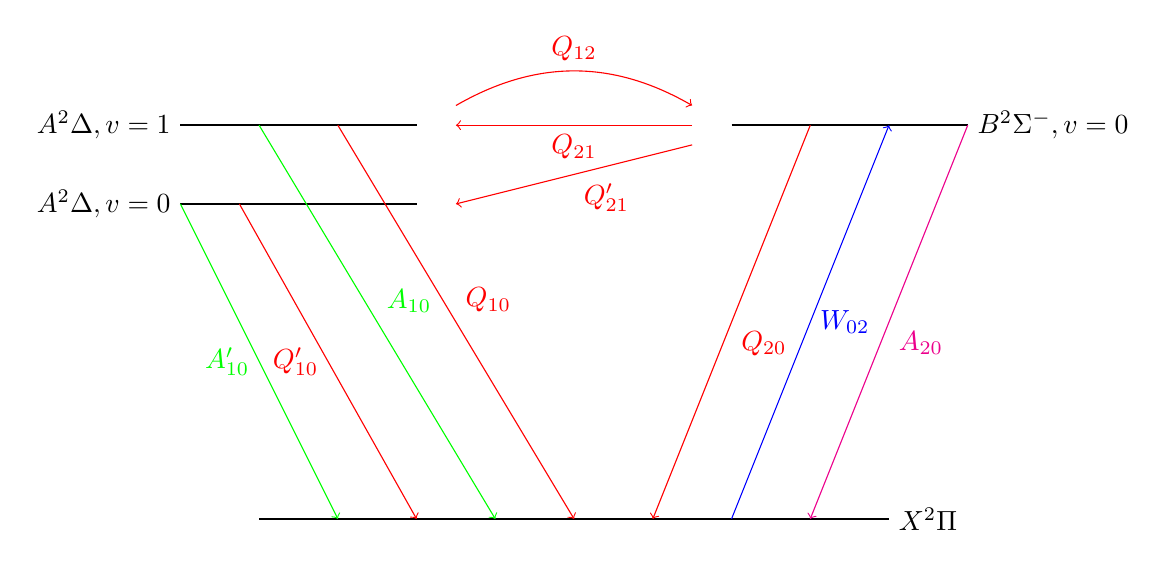
\begin{tikzpicture}

% Ground state
\draw [thick] ( 1, 0 ) -- ++( 8, 0 );
\node at ( 9, 0 ) [right] {\(X^2\Pi\)};

% First electronic states
\draw [thick] ( 0, 4 ) -- ++( 3, 0 );
\node at ( 0, 4 ) [left] {\(A^2\Delta, v = 0\)};
\draw [thick] ( 0, 5 ) -- ++( 3, 0 );
\node at ( 0, 5 ) [left] {\(A^2\Delta, v = 1\)};

% Second electronic state
\draw [thick] ( 7, 5 ) -- ++( 3, 0 );
\node at ( 10, 5 ) [right] {\(B^2\Sigma^-, v = 0\)};

% Transitions
\path [->, blue] ( 7, 0 ) edge node [right] {\(W_{02}\)} ++( 2, 5 );
\path [->, red] ( 8, 5 ) edge node [auto] {\(Q_{20}\)} ++( -2, -5 );
\path [->, magenta] ( 10, 5 ) edge node [auto] {\(A_{20}\)} ++( -2, -5 );

\path [->, red] ( 6.5, 5 ) edge node [auto] {\(Q_{21}\)} ++( -3, 0 );
\path [->, red] ( 6.5, 4.75 ) edge node [auto] {\(Q'_{21}\)} ++( -3, -0.75 );
\path [->, red] ( 3.5, 5.25 ) edge [bend left] node [above] {\(Q_{12}\)} ++( 3, 0 );

\path [->, red] ( 2, 5 ) edge node [auto] {\(Q_{10}\)} ++( 3, -5 );
\path [->, green] ( 1, 5 ) edge node [auto] {\(A_{10}\)} ++( 3, -5 );

\path [->, red] ( 0.75, 4 ) edge node [left] {\(Q'_{10}\)} ++( 2.25, -4 );
\path [->, green] ( 0, 4 ) edge node [left] {\(A'_{10}\)} ++( 2, -4 );

\end{tikzpicture}

\caption[Transitions in the improved CH fluorescence model]{A simplified model of the transitions between the energy levels in a CH system. Excitation (\textcolor{blue}{blue}) of ground state CH molecules to the upper electronic state is followed by several collisional energy transfer processes (\textcolor{red}{red}). A small portion of these molecules spontaneously emit a photon (\textcolor{green}{green}) and return to ground state. The spontaneous emission corresponding to resonant PLIF (\textcolor{magenta}{magenta}) is not collected.}

\label{fig:simplifiedEnergyLevels}

\end{figure}



The rates of the various transition processes are indicated in Figure \ref{fig:simplifiedEnergyLevels}.
\(W_{02}\) is the pumping process that populates the \(B\)(0) state.
\(Q_{ij}\) are collisional energy transfer processes that transfer CH molecules from the \(i\) level to the \(j\) level.
The subscripts 0, 1 and 2 represent the electronic energy levels \(X\), \(A\) and \(B\).
Processes involving the \(A\)(0) state are differentiated from those involving the \(A\)(1) state by a prime (\('\)).
Finally, \(A_{ij}\) represents the spontaneous emission coefficients between the \(i\) and \(j\) levels.

Applying Equation \ref{eqn:fluorescencePhotons} to this case, we can write an expression for the LIF signal intensity as follows,

\begin{equation}
  \Phi = ( n_1 A_{10} + n'_1 A'_{10} )V
  \label{eqn:signalIntensity}
\end{equation}

Our task is to solve for the values of \(n_1\) and \(n'_1\) in terms of \(n_0\).
To do this we need to write rate equations describing the variation of the populations of the three upper states with time.

\begin{align}
  \frac{dn_1}{dt} &= -( A_{10} + Q_{10} + Q_{12} )n_1 + Q_{21} n_2
  \label{eqn:rates1}\\
  \frac{dn'_1}{dt} &= -( A'_{10} + Q'_{10} )n'_1 + Q'_{21} n_2
  \label{eqn:rates2}\\
  \frac{dn_2}{dt} &= W_{02} n_0 + Q_{12} n_1 - ( A_{20} + Q_{20} + Q_{21} + Q'_{21} )n_2
  \label{eqn:rates3}
\end{align}

Under the assumption that the laser excitation time scale is much longer that the collisional time scales, we can set the LHS of Equations \ref{eqn:rates1}--\ref{eqn:rates3} to zero.
This results in a closed set of linear equations, which can be expressed in matrix form as follows.

\begin{equation}
  \left[
    \begin{matrix}
      A_{10} + Q_{10} + Q_{12} & 0 & -Q_{21}\\
      0 & A'_{10} + Q'_{10} & -Q'_{21}\\
      -Q_{12} & 0 & A_{20} + Q_{20} + Q_{21} + Q'_{21}
    \end{matrix}
  \right]\left[
    \begin{matrix}
      n_1\\
      n'_1\\
      n_2
    \end{matrix}
  \right] = \left[
    \begin{matrix}
      0\\
      0\\
      W_{02}n_0
    \end{matrix}
  \right]
  \label{eqn:closedForm}
\end{equation}

From Equation \ref{eqn:closedForm}, we only need the solutions to \(n_1\) and \(n'_1\).
These solutions are presented in Equations \ref{eqn:solution1}--\ref{eqn:solution2}.

\begin{align}
  n_1 &= n_0W_{02}Y
  \label{eqn:solution1}\\
  n'_1 &= n_0W_{02}Y'
  \label{eqn:solution2}
\end{align}.

The expressions for the respective flourescence yields, \(Y\) and \(Y'\) are as follows,

\begin{align}
  Y &= \frac{ Q_{21} }{ ( A_{10} + Q_{10} + Q_{12} )( A_{20} + Q_{20} + Q_{21} + Q'_{21} ) - Q_{12}Q_{21} }
  \label{eqn:flourescenceYield1-unsimplified}\\
  Y' &= \frac{ ( A_{10} + Q_{10} + Q_{12} )Q'_{21} }{ ( A'_{10} + Q'_{10} ) ( ( A_{10} + Q_{10} + Q_{12} )( A_{20} + Q_{20} + Q_{21} + Q'_{21} ) - Q_{12}Q_{21} ) }
  \label{eqn:fluorescenceYield2-unsimplified}
\end{align}

\subsubsection{Solution}
\label{subsubsec:improved-model-solution}

Substituting the expressions from Equations \ref{eqn:solution1}--\ref{eqn:solution2} into Equation \ref{eqn:signalIntensity},

\begin{equation}
  \Phi = n_0VW_{02}(Y + Y')
  \label{eqn:improvedModel-weak}
\end{equation}

Note the similarity in the form of Equation \ref{eqn:improvedModel-weak} to Equation \ref{eqn:twoLevelModel-weak}.
Both expressions are composed of two parts---a pumping rate and a fluorescence yield.
Expanding the pumping rate \(W_{02}\) in a manner identical to Equation \ref{eqn:pumpingRate} and using the absorption integral in Equation \ref{eqn:absorptionIntegral}, we can rewrite Equation \ref{eqn:improvedModel-weak} in a form mirroring Equation \ref{eqn:twoLevelModel}

\begin{equation}
  \Phi = \frac{P}{c} \int_x n_{CH} (Y + Y') \sum_j f_j B_j \int_\nu \psi(\nu) \phi_j(\nu) d\nu dx
  \label{eqn:improvedModel}
\end{equation}

The expressions for the fluorescence yields, \(Y\) and \(Y'\), still have many variables that have not been tabulated conveniently in literature.
As a result, further simplifications will need to be made on the basis of reported experimental observations.
These simplifications are outside the scope of this chapter and will be introduced in Chapter \ref{ch:chplif} along with the results of applying this model to various reactant mixtures.

